\section{Theorie}
\label{sec:Theorie}
Im vorliegenden Versuch wurde das Relaxationsverhalten eines RC-Stromkreises untersucht.

\subsection{Anwendung einer allgemeinen Relaxationsgleichung auf den RC-Kreis}

Generell treten Relaxationsphänomene in der Physik auf, wenn ein System aus seinem Ausgangszustand ausgelenkt wird und anschließend (ohne Oszillation) in diesen Ausgangszustand zurückkehrt. Dabei ist die Änderung der betrachteten Größe zu einer bestimmten Zeit in der Regel proportional zu der Differenz der Größe von ihrem Endzustand. Die Änderung der Größe A kann also mit der Gleichung
\begin{equation}
    \frac{\text{d}A}{\text{d}t} = c \left[A(t) - A(\infty) \right]
    \label{eqn:Relaxation}
\end{equation}
berechnet werden. Eine Umformung (Trennung von dA und dt) und Integration von \autoref{eqn:Relaxation} über die Zeit von 0 bis t ergibt
\begin{equation}
    ln(\frac{A(t) - A(\infty)}{A(0) - A(\infty)}) = c t \text{.}
    \label{eqn:RelaxationInt}
\end{equation}
Die Umformung von \autoref{eqn:RelaxationInt} nach $A(t)$ liefert schließlich 
\begin{equation}
    A(t)= A(\infty)+(A(0) - A(\infty)) e^{c t} \text{.}
    \label{eqn:Auslenkung}
\end{equation}

Als Beispiele für solche Relaxationsvorgänge werden nun die Ent- und die Aufladung eines Kondensators über einen Widerstand betrachtet (siehe \autoref{fig:entaufladung}).
\begin{figure}
    \centering
    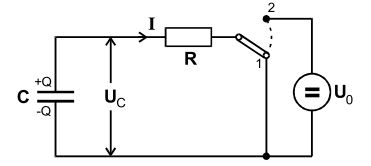
\includegraphics{images/entaufladung.JPG}
    \caption{Beispielschaltung zur Entladung (Stellung 1) und Aufladung (Stellung 2) eines Kondensators über einen Widerstand \cite{VA}}
    \label{fig:entaufladung}
\end{figure}

\textbf{Entladung}:
Wie in \autoref{fig:entaufladung} zu sehen, befindet sich auf den Platten des Kondensators mit Kapazität C die Ladung Q, sodass zwischen den Platten die Spannung $U_C$ liege, die nach 
\begin{equation}
    U_C = \frac{Q}{C}
    \label{eqn:U}
\end{equation}

berechnet werden kann. Das ohmsche Gesetz liefert nun den Strom I durch den Widerstand R, der durch die Spannung hervorgerufen wird:
\begin{equation}
    I =   \frac{U_C}{R}
    \label{eqn:I}
\end{equation}
Der Strom I bewirkt einen Ladungsfluss, sodass sich die Ladung auf den Kondensatorplatten im Zeitintervall dt um
\begin{equation}
    \text{d}Q = -I \text{d}t
    \label{eqn:dQ}
\end{equation}
ändert. Mit \autoref{eqn:U}, \autoref{eqn:I} und \autoref{eqn:dQ} kann nun eine Differentialgleichung für die Ladung auf den Kondensatorplatten $Q(t)$ aufgestellt werden, die die gleiche Form wie \autoref{eqn:Relaxation} hat:
\begin{equation}
        \frac{\text{d}Q}{\text{d}t}  = - \frac{1}{RC} Q(t) 
\end{equation}

Für die Entladung kann angenommen werden, dass $Q(\infty)=0$ gilt. Dann liefert \autoref{eqn:Auslenkung} hier \newline
\begin{equation}
    Q(t)= Q(0) e^{\frac{-t}{RC}} \text{.}
    \label{eqn:Qentl}
\end{equation}


\textbf{Aufladung}:
Der Aufladevorgang des Kondensators kann analog betrachtet werden. Für die Aufladung gelten die Randbedingungen $Q(0)=0$ und $Q(\infty)=CU_0$. Für den zeitlichen Verlauf der Ladung ergibt sich hier also (siehe auch \autoref{eqn:Auslenkung}):
\begin{equation}
    Q(t)= CU_0 (1-e^{\frac{-t}{RC}}) 
    \label{eqn:Qaufl}
\end{equation}
Der Ausdruck $RC$ wird auch als Zeitkonstante des Relaxationsvorganges bezeichnet.

\subsection{Relaxation unter periodischer Auslenkung aus der Gleichgewichtslage}
Die unter periodischer Auslenkung auftretenden Relaxationsphänomene eines RC-Stromkreises werden nun beispielhaft anhand der Schaltung in \autoref{fig:schaltung} betrachtet.

\begin{figure}
    \centering
    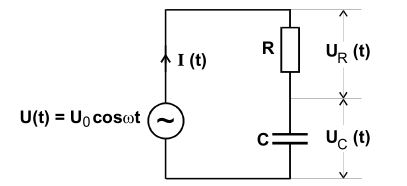
\includegraphics{images/Schaltung.JPG}
    \caption{Beispielschaltung für einen RC-Kreis mit periodischer Anregung \cite{VA}}
    \label{fig:schaltung}
\end{figure}
Wenn die Kreisfrequenz $ \omega << 1/RC$ ist, ist die äußere Wechselspannung  
\begin{equation}
    U(t) = U_0 \cdot \text{cos}(\omega t)
\end{equation}
zu jedem Zeitpunkt praktisch gleich der Spannung am Kondensator $U_C$. Bei steigender Frequenz entsteht allerdings eine Phasenverschiebung zwischen Generator- und Kondensatorspannung, außerdem sinkt die Amplitude der Kondensatorspannung. Im Folgenden werden Formeln für die Frequenzabhängigkeit der Phase $\varphi(\omega)$ und der Amplitude $A(\omega)$ hergeleitet. Für die genauere Betrachtung dieses Zusammenhangs wird der Ansatz
\begin{equation} 
    U_\text{C}(t) = A(\omega) \text{cos}(\omega t + \varphi(\omega))
    \label{eqn:ansatz}
\end{equation}
gewählt.
Mit dem 2. Kirchhoffschen Gesetz (Maschenregel) gilt für die Schaltung in \autoref{fig:schaltung}
\begin{align}
    \label{eqn:Uta}
    U(t) &= U_R(t) + U_C(t) \\
    \iff     U_0 \cos(\omega t) &= I(t)R +A(\omega) \cos(\omega t + \varphi) 
    \label{eqn:Ut}
\end{align}
und mit \autoref{eqn:U} und \autoref{eqn:dQ} kann man die Stromstärke als
\begin{equation}
    \label{eqn:Stromstaerke}
    I(t) = \frac{\text{d}Q}{\text{d}t} = C \cdot \frac{\text{d}U_\text{C}}{\text{d}t}
\end{equation}
schreiben. Das Einsetzen von \autoref{eqn:ansatz} und \autoref{eqn:Stromstaerke} in \autoref{eqn:Ut} ergibt dann die Gleichung

\begin{equation}
    \label{eqn:gl}
        U_0 \cos(\omega t) = -A  \omega RC \sin(\omega t + \varphi)+
        A \cos(\omega t + \varphi)   \text{.}  
\end{equation}

Aus \autoref{eqn:gl} wird für $\omega t = \frac{\pi}{2}$  
\begin{equation}
    0= - \omega RC \sin(\frac{\pi}{2}+\varphi)+\cos(\frac{\pi}{2}+\varphi)
    \label{eqn:pihalbe}
\end{equation}
und dies kann umgeformt werden zu (mit $\sin(\varphi + \frac{\pi}{2}) = \cos \varphi$ und $\cos(\varphi + \frac{\pi}{2}) = - \sin (\varphi)$):

\begin{align}
    \label{eqn:Phase1}
    \frac{\sin(\varphi)}{\cos(\varphi)} = \tan(\varphi) &= - \omega RC \\
    \iff \varphi(\omega) &= \arctan(- \omega RC)
    \label{eqn:Phase}
\end{align}

Mit $\omega t + \varphi =\frac{\pi}{2}$ kann \autoref{eqn:gl} auch zu 
\begin{align}
        U_0 \cos(\frac{\pi}{2} - \varphi) &= -A  \omega RC \\
        \iff A(\omega) &= - \frac{\sin(\varphi)}{\omega RC} U_0
        \label{eqn:gl1}
    \end{align}
umgeformt werden. Aus \autoref{eqn:Phase1} wird dann unter Benutzung des trigonometrischen Pythagoras (man ersetze beispielsweise $\cos(\varphi)$ durch $\sqrt{1-\sin(\varphi)^2}$)
\begin{equation}
    \sin(\varphi) = \frac{\omega R C}{\sqrt{1 + (\omega RC)^2}}.
    \label{eqn:sin}
\end{equation}
hergeleitet. Schließlich erhält man durch Einsetzen von \autoref{eqn:sin} in \autoref{eqn:gl1}
\begin{equation}
    A(\omega) = \frac{U_0}{\sqrt{1 + \omega^2 R^2 C^2}}.
    \label{eqn:Amplitude}
\end{equation}


Mit \autoref{eqn:Phase} und \autoref{eqn:Amplitude} wurden also Formeln für die Frequenzabhängigkeit der Phase und der Amplitude hergeleitet.

\subsection{RC-Kreis als Integrator}
Unter bestimmten Voraussetzungen kann ein RC-Kreis auch als Integrator dienen. Das heißt, dass er eine zeitlich veränderliche Eingangsspannung integriert. Mit \autoref{eqn:Uta} und \autoref{eqn:Stromstaerke} erhält man:
\begin{equation}
    U(t) = RC \frac{\text{d}U_\text{C}}{\text{d}t} + U_\text{C}(t) 
\label{eqn:ut}
\end{equation} 

Die Voraussetzung ist hier, dass $ω >> 1/RC$ ist, dann ist  $|U_C|<<|U_R|$ und $|U_C|<<|U|$. Daher wird \autoref{eqn:ut} näherungsweise zu:

\begin{align}
U(t) &= RC \cdot \frac{\text{d}U_\text{C}}{\text{d}t} \\
\iff U_\text{C}(t) &= \frac{1}{RC} \int^t_0 U(t') \; \text{d} t'
\end{align}